\section{Thuật toán Skip Search}

\subsection{Đặc điểm chính}

Thuật toán Skip Search là một thuật toán tìm kiếm chuỗi dựa trên việc gom các vị trí xuất hiện của từng ký tự trong mẫu vào các nhóm, gọi là các bucket. Thay vì thử khớp mẫu tại mọi vị trí của văn bản, thuật toán chỉ xét một số vị trí cách nhau $m$ ký tự, từ đó suy ra các vị trí bắt đầu tiềm năng của mẫu trong văn bản.

Skip Search đặc biệt hiệu quả khi mẫu ngắn hơn nhiều so với kích thước bảng chữ cái, vì khi đó nhiều bucket sẽ rỗng và số vị trí cần kiểm tra giảm đáng kể.

Thuật toán có các đặc điểm sau:

\begin{itemize}
    \item sử dụng các bucket lưu vị trí xuất hiện của từng ký tự trong bảng chữ cái;
    \item giai đoạn tiền xử lý có độ phức tạp thời gian và không gian $O(m + \sigma)$;
    \item giai đoạn tìm kiếm có độ phức tạp thời gian $O(nm)$;
    \item số phép kiểm tra ký tự văn bản kỳ vọng là $O(n)$.
\end{itemize}

\subsection{Mô tả thuật toán}

Với mỗi ký tự trong bảng chữ cái, thuật toán tạo một bucket chứa tất cả các vị trí xuất hiện của ký tự đó trong mẫu $x$. Nếu một ký tự xuất hiện $k$ lần trong mẫu, thì bucket tương ứng của ký tự đó sẽ chứa $k$ vị trí. Khi mẫu ngắn hơn nhiều so với kích thước bảng chữ cái, nhiều bucket sẽ rỗng.

Giai đoạn tiền xử lý của thuật toán Skip Search gồm việc tính các bucket cho tất cả các ký tự trong bảng chữ cái. Với mỗi ký tự $c \in \Sigma$, ta có:

\[
z[c] = \left\{ i \mid 0 \leq i \leq m - 1 \text{ và } x[i] = c \right\}
\]

Độ phức tạp thời gian và không gian của giai đoạn tiền xử lý là $O(m + \sigma)$.

Vòng lặp chính trong giai đoạn tìm kiếm xét lần lượt mỗi ký tự thứ $m$ của văn bản, tức là các ký tự $y[j]$. Do đó, số vòng lặp chính xấp xỉ là:

\[
\frac{n}{m}.
\]

Với mỗi ký tự $y[j]$, thuật toán sử dụng các vị trí trong bucket $z[y[j]]$ để xác định các vị trí bắt đầu tiềm năng $p$ của mẫu $x$ trong văn bản $y$. Sau đó, thuật toán so sánh mẫu $x$ với văn bản $y$ bắt đầu tại vị trí $p$, từng ký tự một, cho đến khi xảy ra mismatch hoặc toàn bộ mẫu được khớp.

Thuật toán Skip Search có độ phức tạp thời gian bậc hai trong trường hợp xấu nhất, nhưng số phép kiểm tra ký tự văn bản kỳ vọng là $O(n)$.

\subsection{Cài đặt bằng C++}
\begin{verbatim}
#include <iostream>
#include <vector>
#include <string>
#include <cstring>

using namespace std;

const int ASIZE = 256;

/* ---------- Skip Search Algorithm ---------- */
void SkipSearch(const string &pat, const string &txt) {
    int m = pat.length();
    int n = txt.length();

    if (m == 0 || n < m) {
        return;
    }

    /*
        z[c] là bucket chứa các vị trí i sao cho pat[i] == c.
    */
    vector<vector<int>> z(ASIZE);

    /* Preprocessing */
    for (int i = 0; i < m; ++i) {
        z[(unsigned char)pat[i]].push_back(i);
    }

    /* Searching */
    for (int j = m - 1; j < n; j += m) {
        unsigned char c = (unsigned char)txt[j];

        for (int pos : z[c]) {
            int start = j - pos;

            if (start >= 0 && start <= n - m &&
                memcmp(pat.c_str(), txt.c_str() + start, m) == 0) {
                cout << "Pattern found at index: "
                     << start << endl;
            }
        }
    }
}

/* ---------- Main ---------- */
int main() {
    string text = "ABAAABCDABCABC";
    string pattern = "ABC";

    SkipSearch(pattern, text);

    return 0;
}
\end{verbatim}

\subsection{Kiểm nghiệm thuật toán}

\textbf{Pha tiền xử lý:}

\begin{figure}[H]
    \centering
    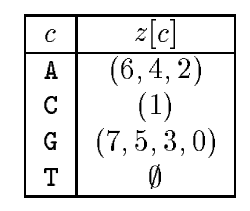
\includegraphics[width=10cm]{Images/2026-05-18-14-30-49.png}
    \caption{Kết quả tiền xử lý (bảng Z) của thuật toán Skip Search}
    \label{fig:skip-search-preprocess}
\end{figure}

Bảng $Z$ sử dụng bởi thuật toán Skip Search.

\textbf{Pha tìm kiếm:}

Lần 1:

\begin{figure}[H]
    \centering
    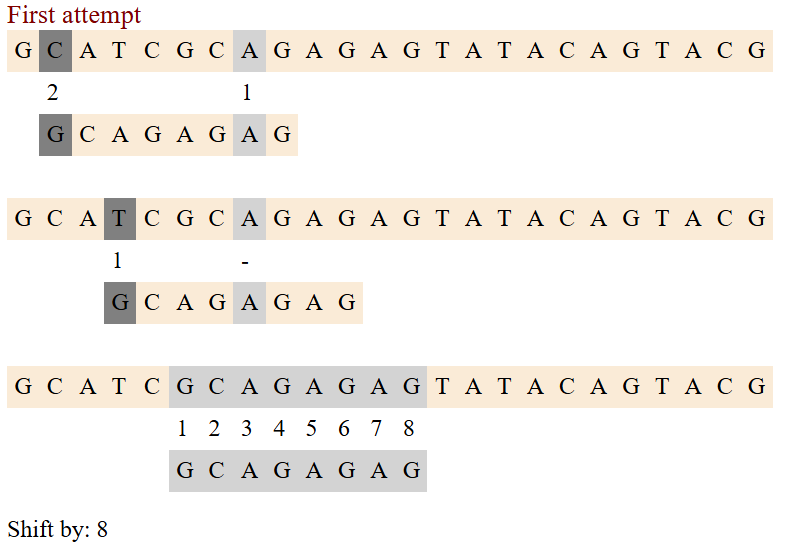
\includegraphics[width=15cm]{Images/2026-05-18-14-31-51.png}
    \caption{Bước 1 trong quá trình thực hiện thuật toán Skip Search}
    \label{fig:skip-search-step-1}
\end{figure}

Lần 2:

\begin{figure}[H]
    \centering
    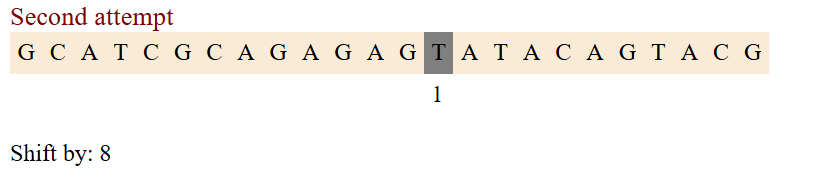
\includegraphics[width=15cm]{Images/2026-05-18-14-32-09.png}
    \caption{Bước 2 trong quá trình thực hiện thuật toán Skip Search}
    \label{fig:skip-search-step-2}
\end{figure}

Lần 3:

\begin{figure}[H]
    \centering
    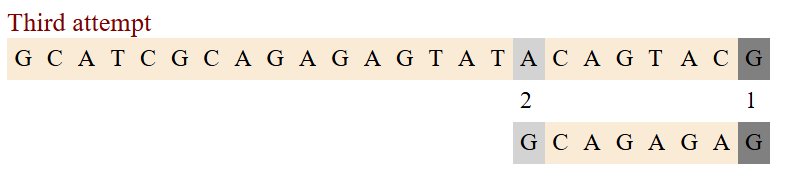
\includegraphics[width=15cm]{Images/2026-05-18-14-32-26.png}
    \caption{Bước 3 trong quá trình thực hiện thuật toán Skip Search}
    \label{fig:skip-search-step-3}
\end{figure}

Thuật toán Skip Search thực hiện 14 lần so khớp chuỗi trong ví dụ trên.

